\chapter{Bit Error Rate (BER)}
\label{ch:ber}

\begin{nontechnical}
\textbf{BER measures how many mistakes happen when transmitting digital data}---like counting typos in a text message.

\textbf{Simple idea:}
\begin{itemize}
\item Wireless signals pick up noise (like static on old radios)
\item Noise can flip bits: 0 becomes 1, or 1 becomes 0
\item BER = fraction of bits that got flipped
\end{itemize}

\textbf{Real examples:}
\begin{itemize}
\item \textbf{Pixelated video}: High BER $\rightarrow$ corrupted data $\rightarrow$ artifacts
\item \textbf{Dropped calls}: BER $> 10^{-3}$ (1 error per 1000 bits) = bad quality
\item \textbf{Corrupted downloads}: Even 1 flipped bit can break a file!
\end{itemize}

\textbf{Acceptable levels:} Voice = $10^{-3}$ OK, Data needs $< 10^{-6}$, Banking requires $< 10^{-12}$

\textbf{Fun fact}: WiFi automatically adjusts speed based on BER---closer = faster (low errors), farther = slower (keep errors acceptable).
\end{nontechnical}

\section{Overview}

\textbf{Bit Error Rate (BER)} is the fundamental performance metric for digital communication systems, quantifying the probability that a transmitted bit is incorrectly received.

\begin{keyconcept}
BER represents the ratio of incorrectly decoded bits to total transmitted bits. It is the primary metric for assessing link quality and determining whether a communication system meets its performance requirements.
\end{keyconcept}

BER forms the foundation for comparing modulation schemes, evaluating error correction techniques, and establishing link budgets for reliable data transmission.

\section{Mathematical Definition}

\subsection{Basic Formula}

The bit error rate is formally defined as:
\begin{equation}
\mathrm{BER} = \frac{N_e}{N_t}
\label{eq:ber-definition}
\end{equation}
where:
\begin{itemize}
\item $N_e$ = number of bit errors detected
\item $N_t$ = total number of bits transmitted
\end{itemize}

\textbf{Alternative expression} as probability:
\begin{equation}
\mathrm{BER} = P_b = P(\hat{b} \neq b)
\label{eq:ber-probability}
\end{equation}
where $b$ is the transmitted bit and $\hat{b}$ is the received bit.

\subsection{BER Scale and Interpretation}

BER is typically expressed in scientific notation spanning many orders of magnitude:

\begin{center}
\begin{tabular}{@{}lll@{}}
\toprule
BER Value & Meaning & Quality \\
\midrule
$10^{-1}$ & 1 error per 10 bits & Terrible \\
$10^{-2}$ & 1 error per 100 bits & Very Poor \\
$10^{-3}$ & 1 error per 1,000 bits & Poor \\
$10^{-4}$ & 1 error per 10,000 bits & Marginal \\
$10^{-6}$ & 1 error per 1,000,000 bits & Good \\
$10^{-9}$ & 1 error per 1 billion bits & Excellent \\
$10^{-12}$ & 1 error per 1 trillion bits & Exceptional \\
\bottomrule
\end{tabular}
\end{center}

\section{Theoretical BER in AWGN Channel}

\subsection{Relationship to Q-Function}

For most coherent modulation schemes in additive white Gaussian noise (AWGN), BER can be expressed using the Gaussian Q-function:
\begin{equation}
Q(x) = \frac{1}{\sqrt{2\pi}} \int_x^\infty e^{-t^2/2}\,dt
\label{eq:q-function}
\end{equation}
where:
\begin{itemize}
\item $Q(x)$ = probability that a standard normal random variable exceeds $x$
\item $x$ = threshold normalized by noise standard deviation
\end{itemize}

\textbf{Complementary error function} representation:
\begin{equation}
Q(x) = \frac{1}{2}\mathrm{erfc}\left(\frac{x}{\sqrt{2}}\right)
\label{eq:q-erfc}
\end{equation}
where $\mathrm{erfc}(x) = \frac{2}{\sqrt{\pi}}\int_x^\infty e^{-t^2}\,dt$ is the complementary error function.

\subsection{BPSK Coherent Detection}

For ideal BPSK with coherent detection in AWGN:
\begin{equation}
\mathrm{BER}_{\mathrm{BPSK}} = Q\left(\sqrt{\frac{2E_b}{N_0}}\right) = \frac{1}{2}\mathrm{erfc}\left(\sqrt{\frac{E_b}{N_0}}\right)
\label{eq:ber-bpsk}
\end{equation}
where:
\begin{itemize}
\item $E_b$ = energy per bit (joules)
\item $N_0$ = noise power spectral density (W/Hz)
\item $E_b/N_0$ = fundamental energy-to-noise ratio (often expressed in dB)
\end{itemize}

\subsection{Other Modulation Schemes}

\textbf{QPSK (coherent):}
\begin{equation}
\mathrm{BER}_{\mathrm{QPSK}} = Q\left(\sqrt{\frac{2E_b}{N_0}}\right)
\label{eq:ber-qpsk}
\end{equation}
(Same as BPSK because each I/Q component is independent)

\textbf{FSK (non-coherent):}
\begin{equation}
\mathrm{BER}_{\mathrm{FSK}} = \frac{1}{2}e^{-E_b/(2N_0)}
\label{eq:ber-fsk}
\end{equation}

\textbf{M-QAM (square constellation):}
\begin{equation}
\mathrm{BER}_{\mathrm{M-QAM}} \approx \frac{4}{\log_2 M}\left(1 - \frac{1}{\sqrt{M}}\right)Q\left(\sqrt{\frac{3\log_2 M}{M-1}\frac{E_b}{N_0}}\right)
\label{eq:ber-mqam}
\end{equation}
where $M$ = number of constellation points.

\section{Pre-FEC vs Post-FEC BER}

\subsection{Pre-FEC (Raw) BER}

The error rate \textbf{before} forward error correction (FEC) decoding:
\begin{equation}
\mathrm{BER}_{\mathrm{raw}} = \frac{N_{e,\mathrm{raw}}}{N_t}
\label{eq:ber-raw}
\end{equation}

Characteristics:
\begin{itemize}
\item Directly reflects channel quality
\item Higher at low SNR
\item Called ``channel BER'' or ``raw BER''
\item Determines FEC decoder input quality
\end{itemize}

\subsection{Post-FEC (Corrected) BER}

The residual error rate \textbf{after} FEC decoding:
\begin{equation}
\mathrm{BER}_{\mathrm{post}} = \frac{N_{e,\mathrm{corrected}}}{N_t}
\label{eq:ber-post}
\end{equation}

Characteristics:
\begin{itemize}
\item Shows effectiveness of error correction
\item Should be much lower than pre-FEC BER
\item Represents ``residual errors'' that couldn't be corrected
\item Final system performance metric
\end{itemize}

\subsection{Coding Gain}

The improvement provided by FEC is quantified as:
\begin{equation}
G_{\mathrm{coding}} = 10\log_{10}\left(\frac{\mathrm{BER}_{\mathrm{raw}}}{\mathrm{BER}_{\mathrm{post}}}\right) \text{ dB}
\label{eq:coding-gain}
\end{equation}

\begin{calloutbox}{Example: LDPC Coding Gain}
\textbf{Scenario:} LDPC(1024,512) code with rate $R = 1/2$

\begin{tabular}{@{}ll@{}}
Pre-FEC BER: & $10^{-2}$ (1 error per 100 bits) \\
Post-FEC BER: & $10^{-6}$ (1 error per million bits) \\
Coding Gain: & $40$ dB improvement \\
\end{tabular}

This represents a $10,000\times$ reduction in error rate, achieved by adding redundancy (doubling the required bandwidth for rate 1/2 code).
\end{calloutbox}

\section{BER Performance Curves}

\subsection{BER vs $E_b/N_0$ Characteristic}

The fundamental performance plot for digital communication systems shows BER as a function of $E_b/N_0$:

\begin{center}
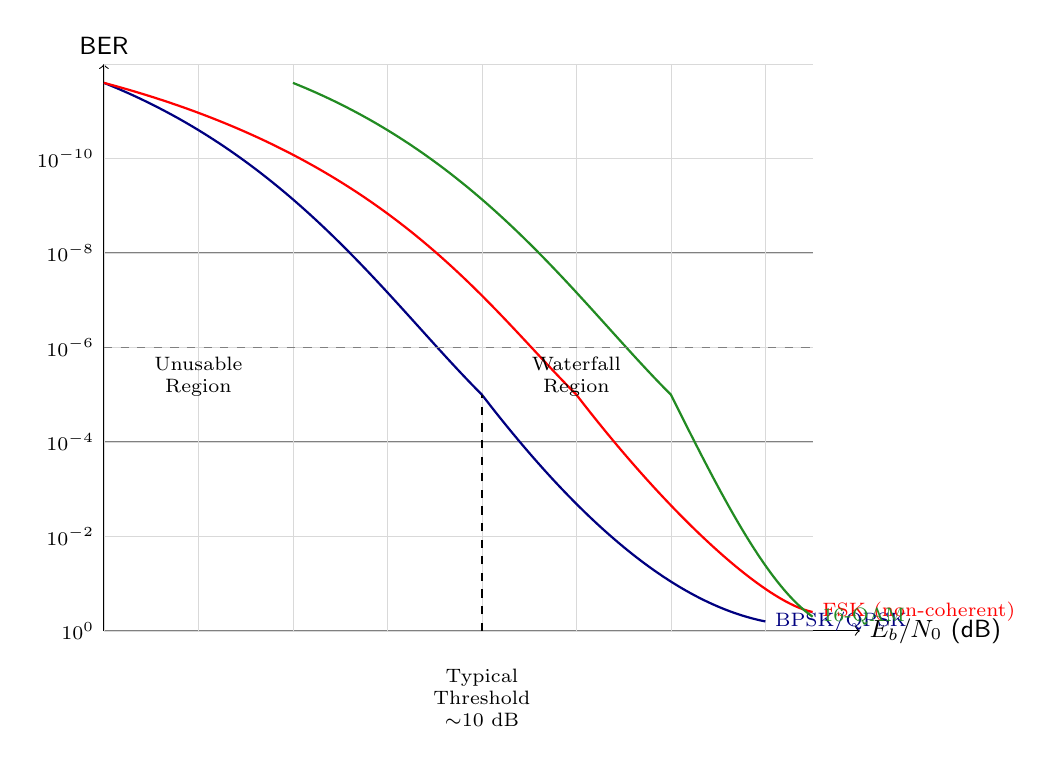
\begin{tikzpicture}[scale=1.2]
% Axes with logarithmic BER scale
\draw[->] (0,0) -- (8,0) node[right] {\sffamily\small $E_b/N_0$ (dB)};
\draw[->] (0,0) -- (0,6) node[above] {\sffamily\small BER};

% Logarithmic scale labels on y-axis
\foreach \y/\label in {0/$10^{0}$, 1/$10^{-2}$, 2/$10^{-4}$, 3/$10^{-6}$, 4/$10^{-8}$, 5/$10^{-10}$} {
    \draw[thin,gray] (0,\y) -- (7.5,\y);
    \node[left,font=\scriptsize] at (0,\y) {\label};
}

% Grid
\draw[very thin,gray!30] (0,0) grid[xstep=1,ystep=1] (7.5,6);

% BPSK curve (steepest)
\draw[thick,NavyBlue] (0,5.8) .. controls (2,5) and (3,3.5) .. (4,2.5) .. controls (5,1.2) and (6,0.3) .. (7,0.1);
\node[right,NavyBlue,font=\scriptsize] at (7,0.1) {BPSK/QPSK};

% FSK curve (shifted right ~3 dB)
\draw[thick,Red] (0,5.8) .. controls (3,5) and (4,3.5) .. (5,2.5) .. controls (6,1.2) and (7,0.3) .. (7.5,0.2);
\node[right,Red,font=\scriptsize] at (7.5,0.2) {FSK (non-coherent)};

% 16-QAM curve (better at high SNR, worse at low)
\draw[thick,ForestGreen] (2,5.8) .. controls (4,5) and (5,3.5) .. (6,2.5) .. controls (6.5,1.5) and (7,0.5) .. (7.5,0.15);
\node[right,ForestGreen,font=\scriptsize] at (7.5,0.15) {16-QAM};

% Regions
\draw[dashed,gray] (0,3) -- (7.5,3);
\node[below,font=\scriptsize,align=center] at (1,3) {Unusable\\Region};
\node[below,font=\scriptsize,align=center] at (5,3) {Waterfall\\Region};

% Threshold annotation
\draw[dashed,thick] (4,0) -- (4,2.5);
\node[below,font=\scriptsize,align=center] at (4,-0.3) {Typical\\Threshold\\$\sim$10 dB};

\end{tikzpicture}
\end{center}

\subsection{Key Features of BER Curves}

\textbf{Waterfall Region:}
The steep decrease in BER as $E_b/N_0$ increases characterizes the transition from unusable to reliable communication:
\begin{equation}
\frac{d(\log_{10} \mathrm{BER})}{d(E_b/N_0)} \approx -0.4 \text{ to } -0.6 \text{ per dB}
\label{eq:ber-slope}
\end{equation}

This means BER typically improves by \textbf{one order of magnitude} (factor of 10) for every 2--3 dB increase in $E_b/N_0$.

\textbf{Operating Threshold:}
The $E_b/N_0$ value where BER becomes acceptable for the application (commonly $10^{-6}$ for data):
\begin{itemize}
\item BPSK: 10.5 dB for BER = $10^{-6}$
\item QPSK: 10.5 dB for BER = $10^{-6}$ (same as BPSK)
\item FSK (non-coherent): 13.5 dB for BER = $10^{-6}$ (3 dB penalty)
\item 16-QAM: 14.5 dB for BER = $10^{-6}$ (requires higher SNR)
\end{itemize}

\textbf{Error Floor:}
The minimum achievable BER due to implementation imperfections:
\begin{equation}
\mathrm{BER}_{\mathrm{floor}} = \lim_{E_b/N_0 \to \infty} \mathrm{BER}
\label{eq:ber-floor}
\end{equation}

Causes include:
\begin{itemize}
\item Quantization noise in ADC/DAC
\item Phase noise in oscillators
\item IQ imbalance
\item Residual intersymbol interference (ISI)
\end{itemize}

\subsection{Q-Function Visualization}

The Gaussian Q-function determines error probability for coherent detection:

\begin{center}
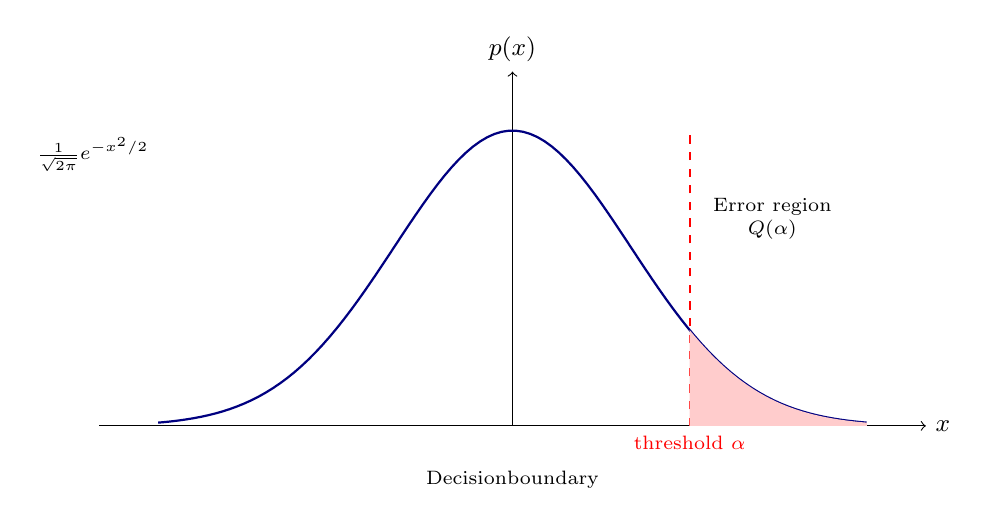
\begin{tikzpicture}[scale=1.5]
% Gaussian PDF
\draw[->] (-3.5,0) -- (3.5,0) node[right] {\sffamily\small $x$};
\draw[->] (0,0) -- (0,3) node[above] {\sffamily\small $p(x)$};

% Gaussian curve
\draw[thick,NavyBlue,domain=-3:3,samples=100] plot (\x,{2.5*exp(-\x*\x/2)});

% Threshold line
\draw[thick,dashed,red] (1.5,0) -- (1.5,2.5);
\node[below,red,font=\scriptsize] at (1.5,0) {threshold $\alpha$};

% Shaded error region
\fill[red!20,domain=1.5:3,samples=50] (1.5,0) -- plot (\x,{2.5*exp(-\x*\x/2)}) -- (3,0) -- cycle;

% Labels
\node[above,font=\scriptsize,align=center] at (2.2,1.5) {Error region\\$Q(\alpha)$};
\node[below,font=\scriptsize] at (0,-0.3) {Decision\\boundary};

% Axes labels
\node[left,font=\scriptsize] at (-3,2.3) {$\frac{1}{\sqrt{2\pi}}e^{-x^2/2}$};

\end{tikzpicture}
\end{center}

The shaded area represents $Q(\alpha) = P(\text{error})$ when the decision threshold is at $\alpha$ standard deviations from the mean.

\subsection{Theoretical vs Measured BER}

\subsubsection{Theoretical BER}

Based on analytical formulas (e.g., Equation~\ref{eq:ber-bpsk} for BPSK):
\begin{itemize}
\item Assumes ideal hardware (infinite precision)
\item Perfect synchronization (carrier, timing, frame)
\item Pure AWGN channel (no fading, no interference)
\item Optimal detection (matched filter, maximum likelihood)
\end{itemize}

\subsubsection{Measured BER}

Actual errors observed in simulation or hardware:
\begin{equation}
\mathrm{BER}_{\mathrm{measured}} = \frac{\text{errors counted}}{\text{bits transmitted}}
\label{eq:ber-measured}
\end{equation}

\textbf{Confidence interval} for measured BER (95\% confidence):
\begin{equation}
\mathrm{BER}_{\mathrm{measured}} \pm 1.96\sqrt{\frac{\mathrm{BER}_{\mathrm{measured}}(1-\mathrm{BER}_{\mathrm{measured}})}{N_t}}
\label{eq:ber-confidence}
\end{equation}

\begin{warningbox}
To measure BER = $10^{-6}$ with reasonable confidence, you must transmit \textbf{at least $10^7$ to $10^8$ bits}. At 1~Mbps, this requires 10--100 seconds. For lower BER targets ($10^{-9}$ or better), measurement time becomes prohibitively long, making simulation or extrapolation necessary.
\end{warningbox}

\subsubsection{Sources of Discrepancy}

Differences between theoretical and measured BER:
\begin{itemize}
\item \textbf{Implementation loss}: Finite precision, non-ideal filters (typically 1--3 dB)
\item \textbf{Synchronization errors}: Imperfect carrier/timing recovery ($\sim$0.5--2 dB)
\item \textbf{Channel model mismatch}: Real channels differ from AWGN
\item \textbf{Finite sample size}: Statistical variation in measurements
\end{itemize}

\section{Factors Affecting BER}

\subsection{Signal-to-Noise Ratio (SNR)}

The \textbf{primary determinant} of BER. For AWGN channels:
\begin{equation}
\mathrm{BER} \propto Q\left(\sqrt{k \cdot \frac{E_b}{N_0}}\right)
\label{eq:ber-snr-relation}
\end{equation}
where $k$ depends on modulation scheme (typically $k = 1$ to $k = 2$).

Higher SNR $\rightarrow$ lower BER (exponentially in many cases).

\subsection{Modulation Scheme}

Different modulations have different noise immunity:

\begin{center}
\begin{tabular}{@{}llc@{}}
\toprule
Modulation & BER Formula & Rel. to BPSK \\
\midrule
BPSK & $Q(\sqrt{2E_b/N_0})$ & 0 dB \\
QPSK & $Q(\sqrt{2E_b/N_0})$ & 0 dB \\
8-PSK & $\approx 2Q(\sqrt{6E_s/N_0}\sin(\pi/8))$ & +4 dB \\
16-QAM & $\approx 3Q(\sqrt{4E_s/(5N_0)})$ & +4--6 dB \\
64-QAM & Complex & +8--10 dB \\
\bottomrule
\end{tabular}
\end{center}

\textbf{Trade-off:} Higher-order modulations (16-QAM, 64-QAM) achieve better spectral efficiency but require higher $E_b/N_0$ for the same BER.

\subsection{Forward Error Correction (FEC)}

FEC codes add redundancy to detect and correct errors:
\begin{equation}
\mathrm{BER}_{\mathrm{coded}} \ll \mathrm{BER}_{\mathrm{uncoded}}
\label{eq:ber-fec}
\end{equation}

\textbf{Common FEC schemes:}
\begin{itemize}
\item \textbf{Reed-Solomon:} Block code, excellent burst error correction
\item \textbf{Convolutional:} Stream processing, moderate performance
\item \textbf{Turbo codes:} Near Shannon-limit performance (0.5--1 dB gap)
\item \textbf{LDPC codes:} Near Shannon-limit, flexible structure, widely used
\item \textbf{Polar codes:} Provably capacity-achieving, 5G standard
\end{itemize}

\subsection{Channel Impairments}

Real-world effects that degrade BER:

\textbf{Multipath fading:}
\begin{equation}
\mathrm{BER}_{\mathrm{fading}} = \int_0^\infty \mathrm{BER}(\gamma) \cdot p(\gamma)\,d\gamma
\label{eq:ber-fading}
\end{equation}
where $p(\gamma)$ is the fading distribution (Rayleigh, Rician, etc.).

\textbf{Interference:} Co-channel or adjacent channel interference increases effective noise:
\begin{equation}
\frac{E_b}{N_0 + I_0}
\label{eq:eb-n0-interference}
\end{equation}

\textbf{Phase noise:} Random phase fluctuations cause constellation rotation, increasing symbol errors.

\textbf{Frequency offset:} Doppler shift or oscillator mismatch causes IQ rotation and ISI.

\subsection{Implementation Imperfections}

\textbf{Quantization:} Limited ADC/DAC resolution adds noise:
\begin{equation}
\mathrm{SNR}_{\mathrm{quantization}} \approx 6.02b + 1.76 \text{ dB}
\label{eq:snr-quantization}
\end{equation}
where $b$ = number of bits in ADC/DAC.

\textbf{Synchronization errors:}
\begin{itemize}
\item Timing offset: Sampling away from optimal instant
\item Carrier phase error: Reduces signal projection
\item Frame misalignment: Corrupts symbol boundaries
\end{itemize}

\textbf{Hardware nonlinearities:} Amplifier compression, mixer imbalance, filter distortion.

\section{Worked Example: Link Budget with BER Target}

\textbf{Scenario:} Design a satellite downlink to achieve BER = $10^{-6}$ using QPSK modulation.

\subsection*{Given Parameters}

\begin{tabular}{@{}ll@{}}
Transmit power & $P_t = 20$ W = 43 dBm \\
TX antenna gain & $G_t = 25$ dBi \\
Distance & $d = 36{,}000$ km (GEO orbit) \\
Frequency & $f = 4$ GHz (C-band downlink) \\
RX antenna gain & $G_r = 35$ dBi (2.4 m dish) \\
System noise temp & $T_s = 200$ K \\
Data rate & $R_b = 2$ Mbps \\
Required BER & $10^{-6}$ \\
\end{tabular}

\subsection*{Step 1: Required $E_b/N_0$ for Target BER}

For QPSK in AWGN, from Equation~\ref{eq:ber-qpsk}:
\begin{equation}
10^{-6} = Q\left(\sqrt{\frac{2E_b}{N_0}}\right)
\end{equation}

Solving numerically (or using Q-function tables):
\begin{equation}
\sqrt{\frac{2E_b}{N_0}} \approx 4.75 \quad \Rightarrow \quad \frac{E_b}{N_0} = 11.3 \text{ (linear)} = 10.5 \text{ dB}
\end{equation}

\subsection*{Step 2: Free-Space Path Loss}

\begin{equation}
\mathrm{FSPL} = 20\log_{10}(d_{\text{km}}) + 20\log_{10}(f_{\text{MHz}}) + 32.45
\end{equation}
\begin{equation}
\mathrm{FSPL} = 20\log_{10}(36{,}000) + 20\log_{10}(4{,}000) + 32.45 = 196.0 \text{ dB}
\end{equation}

\subsection*{Step 3: Received Signal Power}

\begin{equation}
P_r = P_t + G_t + G_r - \mathrm{FSPL}
\end{equation}
\begin{equation}
P_r = 43 + 25 + 35 - 196 = -93 \text{ dBm}
\end{equation}

\subsection*{Step 4: Noise Power}

\begin{equation}
N = kT_sB = (1.38 \times 10^{-23})(200)(2 \times 10^6) = 5.52 \times 10^{-15} \text{ W}
\end{equation}
\begin{equation}
N = 10\log_{10}(5.52 \times 10^{-15} / 10^{-3}) = -112.6 \text{ dBm}
\end{equation}

\subsection*{Step 5: Received SNR}

\begin{equation}
\mathrm{SNR} = P_r - N = -93 - (-112.6) = 19.6 \text{ dB}
\end{equation}

\subsection*{Step 6: Convert SNR to $E_b/N_0$}

For QPSK with 2 bits/symbol:
\begin{equation}
\frac{E_b}{N_0} = \mathrm{SNR} + 10\log_{10}\left(\frac{B}{R_b}\right)
\end{equation}

Assuming Nyquist bandwidth $B \approx R_b = 2$ MHz:
\begin{equation}
\frac{E_b}{N_0} = 19.6 + 10\log_{10}(1) = 19.6 \text{ dB}
\end{equation}

\subsection*{Step 7: Link Margin}

\begin{equation}
\text{Margin} = \frac{E_b}{N_0}_{\text{available}} - \frac{E_b}{N_0}_{\text{required}} = 19.6 - 10.5 = 9.1 \text{ dB}
\end{equation}

\begin{calloutbox}[colback=black!8!white,colframe=black]{Link Budget Summary}
\textbf{Result: Link achieves BER = $10^{-6}$ with 9.1 dB margin}

This margin accommodates:
\begin{itemize}
\item Rain fade (4--6 dB at C-band)
\item Implementation loss (2--3 dB)
\item Pointing errors (1--2 dB)
\item Component aging
\end{itemize}

\textbf{Conclusion:} The link design is viable with reasonable margin for adverse conditions.
\end{calloutbox}

\section{Acceptable BER Thresholds}

Different applications have different BER requirements based on their tolerance for errors:

\begin{center}
\begin{tabular}{@{}lll@{}}
\toprule
Application & Required BER & Rationale \\
\midrule
Voice (analog) & $10^{-3}$ & Some crackling acceptable \\
Data (with retransmission) & $10^{-4}$ to $10^{-6}$ & Retries handle errors \\
Streaming video & $10^{-6}$ & Occasional glitch OK \\
File transfer & $10^{-9}$ & Data integrity critical \\
Financial transactions & $< 10^{-12}$ & Zero tolerance \\
\bottomrule
\end{tabular}
\end{center}

\begin{keyconcept}
The required BER is determined by the application's error sensitivity and whether higher-layer protocols (e.g., TCP retransmission) can recover from errors. Real-time applications (voice, video) have relaxed BER requirements because retransmission causes unacceptable latency.
\end{keyconcept}

\section{Applications}

\subsection{Satellite Communications}

BER is the primary quality metric for satellite links:
\begin{itemize}
\item \textbf{DVB-S2 standard}: Requires BER $< 10^{-7}$ after FEC for video broadcasting
\item \textbf{Target BER}: $10^{-11}$ to $10^{-12}$ for data services
\item \textbf{Link design}: Margins sized to maintain target BER during rain fade
\item \textbf{Adaptive coding}: Modulation/code rate adjusted dynamically based on measured BER
\end{itemize}

\subsection{Wireless Standards (LTE, 5G)}

BER determines block error rate (BLER) and throughput:
\begin{itemize}
\item \textbf{LTE PDSCH}: Target BLER = 10\% at SNR operating point
\item \textbf{5G NR}: Ultra-reliable low-latency (URLLC) requires BER $< 10^{-9}$
\item \textbf{Link adaptation}: Modulation and coding scheme (MCS) selected to maximize throughput while maintaining BER target
\item \textbf{HARQ}: Hybrid ARQ retransmits blocks that fail CRC (driven by residual BER)
\end{itemize}

\subsection{Optical Fiber Communications}

Ultra-high-speed systems ($>$ 100 Gbps) have stringent BER requirements:
\begin{itemize}
\item \textbf{Standard}: ITU-T G.975.1 specifies BER $< 10^{-12}$ pre-FEC
\item \textbf{FEC}: Reed-Solomon or LDPC reduces BER to $< 10^{-15}$
\item \textbf{Measurement}: Real-time BER monitoring for link health
\item \textbf{Challenge}: Achieving low BER at high symbol rates with chromatic dispersion and PMD
\end{itemize}

\subsection{Deep Space Communications}

Extreme path loss demands optimal BER performance:
\begin{itemize}
\item \textbf{NASA Deep Space Network}: Uses concatenated coding (convolutional + Reed-Solomon) to achieve BER $< 10^{-6}$ at very low $E_b/N_0$
\item \textbf{Voyager probes}: Operate at $E_b/N_0 \approx 3$--5 dB with coding gain of 7--9 dB
\item \textbf{Trade-off}: Lower data rates (bits/sec) to maintain acceptable BER with limited power
\end{itemize}

\section{BER Measurement Techniques}

\subsection{Direct Error Counting}

Transmit known test pattern and count mismatches:
\begin{equation}
\mathrm{BER}_{\mathrm{est}} = \frac{N_{\mathrm{errors}}}{N_{\mathrm{bits}}}
\end{equation}

\textbf{Block diagram of BER test system:}

\begin{center}
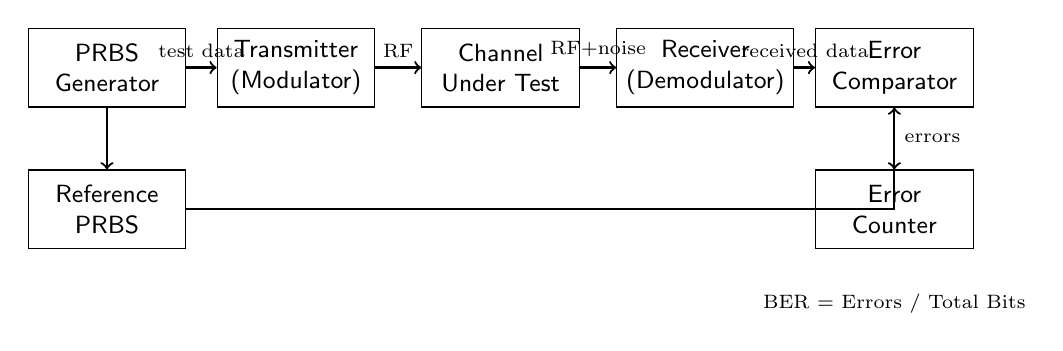
\begin{tikzpicture}[
  block/.style={rectangle, draw, minimum width=2cm, minimum height=1cm, font=\sffamily\small, align=center},
  node distance=2cm,
  font=\small
]
% Transmitter side
\node (prbs) [block] {PRBS\\Generator};
\node (tx) [block, right of=prbs, node distance=2.4cm] {Transmitter\\(Modulator)};
\node (channel) [block, right of=tx, node distance=2.6cm] {Channel\\Under Test};

% Receiver side
\node (rx) [block, right of=channel, node distance=2.6cm] {Receiver\\(Demodulator)};
\node (comp) [block, right of=rx, node distance=2.4cm] {Error\\Comparator};
\node (counter) [block, below of=comp, node distance=1.8cm] {Error\\Counter};

% Reference path
\node (ref) [block, below of=prbs, node distance=1.8cm] {Reference\\PRBS};

% Connections
\draw[->,thick] (prbs) -- node[above,font=\scriptsize] {test data} (tx);
\draw[->,thick] (tx) -- node[above,font=\scriptsize] {RF} (channel);
\draw[->,thick] (channel) -- node[above,font=\scriptsize] {RF+noise} (rx);
\draw[->,thick] (rx) -- node[above,font=\scriptsize] {received data} (comp);
\draw[->,thick] (comp) -- node[right,font=\scriptsize] {errors} (counter);
\draw[->,thick] (prbs) -- (ref);
\draw[->,thick] (ref) -| (comp);

% Labels
\node[below of=counter, node distance=1.2cm, font=\scriptsize, align=center] {BER = Errors / Total Bits};

\end{tikzpicture}
\end{center}

\textbf{Requirements:}
\begin{itemize}
\item Need $\geq 100$ errors for statistical validity
\item For BER = $10^{-6}$: must transmit $\geq 10^8$ bits
\item Test time = $N_{\mathrm{bits}} / R_b$ (e.g., 100 seconds at 1 Mbps)
\end{itemize}

\subsection{Eye Diagram Analysis}

Qualitative BER estimation from oscilloscope:
\begin{itemize}
\item Eye opening correlates with noise margin
\item Larger opening $\rightarrow$ lower BER
\item Quick diagnostic but not quantitative
\end{itemize}

\subsection{Q-Factor Measurement}

Optical communications use Q-factor as BER proxy:
\begin{equation}
Q = \frac{\mu_1 - \mu_0}{\sigma_1 + \sigma_0}
\label{eq:q-factor}
\end{equation}
where $\mu_1, \mu_0$ are mean signal levels for bits 1 and 0, and $\sigma_1, \sigma_0$ are their standard deviations.

Relationship to BER:
\begin{equation}
\mathrm{BER} \approx Q(Q) = \frac{1}{2}\mathrm{erfc}\left(\frac{Q}{\sqrt{2}}\right)
\label{eq:ber-q-factor}
\end{equation}

\section{Summary}

\begin{center}
\begin{tabular}{@{}ll@{}}
\toprule
\textbf{Parameter} & \textbf{Value/Description} \\
\midrule
Definition & Ratio of bit errors to total bits \\
Typical range & $10^{-1}$ (unusable) to $10^{-12}$ (exceptional) \\
Primary dependence & $E_b/N_0$ (energy per bit to noise ratio) \\
BPSK @ BER=$10^{-6}$ & Requires $E_b/N_0 = 10.5$ dB \\
FEC improvement & 10--40 dB coding gain typical \\
Measurement time & $\sim 100/\mathrm{BER}$ bits needed \\
Applications & All digital communications \\
\bottomrule
\end{tabular}
\end{center}

\textbf{Key Insights:}
\begin{itemize}
\item BER is the fundamental metric for digital link quality
\item Exponentially sensitive to $E_b/N_0$ in waterfall region
\item Different applications require vastly different BER targets
\item FEC coding provides massive BER improvements (orders of magnitude)
\item Practical systems balance BER, data rate, and bandwidth
\end{itemize}

\section{Further Reading}

\begin{itemize}
\item For SNR fundamentals: Chapter on Signal-to-Noise Ratio (SNR)
\item For modulation BER comparison: Chapters on BPSK, QPSK, QAM
\item For FEC techniques: Chapter on Forward Error Correction
\item For energy ratios: Chapter on $E_s/N_0$ and $E_b/N_0$
\item For practical measurements: Chapter on Link Budget Analysis
\end{itemize}
